%vim:ft=tex:
%
\documentclass[a4paper,notitlepage]{article}
\usepackage[utf8]{inputenc}
\usepackage[T1]{fontenc}
\usepackage[icelandic]{babel}
\usepackage{fancyhdr}
\usepackage{amsmath}
\usepackage{amssymb}
\usepackage{enumitem}
\usepackage{mdframed}
\usepackage{amsthm}
\usepackage{tikz}
\usepackage{import}
\usepackage{pdfpages}
\usepackage{transparent}
\usepackage{xifthen}
\usepackage{multicol}
\usepackage{float}
\usepackage{graphicx}
\usepackage{pdfpages}
\usepackage{stix}
\usepackage{transparent}
\usepackage[margin=1.5in]{geometry}
\usetikzlibrary{automata,arrows}

\newcommand{\incfig}[1]{%
    \def\svgwidth{\columnwidth}
    \import{./figures/}{#1.pdf_tex}
}

\fancypagestyle{firstpage}{
    \fancyhf{}
    \fancyhead[L]{Fléttufræði \\ 14. september 2021}
    \fancyhead[R]{Tristan Ferrua Edwardsson \\ tfe1@hi.is}
}

\title{Dæmatími, PS2}
\date{}
\author{}

\theoremstyle{plain}
\newmdtheoremenv[innerbottommargin=\topskip]{setning}{Setning}
\theoremstyle{definition}
\newmdtheoremenv[innerbottommargin=\topskip]{skilgr}{Skilgreining}
\newcommand{\wre}{\hrectangle}
\newcommand{\bre}{\hrectangleblack}
\newcommand{\wsq}{\smwhtsquare}

\newmdenv[
  topline=false,
  bottomline=false,
  skipabove=\topsep,
  skipbelow=\topsep
]{siderules}

\fancypagestyle{otherpages}{
    \fancyhf{}
    \fancyhead[L]{\leftmark}
    \fancyhead[R]{\thepage}
}

\newcommand{\quotes}[1]{,,#1''}

\makeatletter
\newcommand{\leqnomode}{\tagsleft@true}
\newcommand{\reqnomode}{\tagsleft@false}
\makeatother

\renewcommand{\labelenumi}{\alph{enumi}.}

\setlength{\parindent}{0ex}

\pagestyle{otherpages}

\DeclareMathOperator*{\adj}{adj}
\DeclareMathOperator*{\nul}{Null}
\DeclareMathOperator*{\col}{Col}
\newcommand{\detmat}[1]{\left|\begin{matrix} #1 \end{matrix}\right|}
\newcommand{\vect}[1]{\left[\begin{array}{r} #1 \end{array}\right]}

\begin{document}

\maketitle
\thispagestyle{firstpage}

\section*{Problem 1.14}
\paragraph{Description:}
\begin{enumerate}
    \item Give a combinotorical proof of the identity
    \begin{equation*}
        \sum_{n=k}^m \binom{n}{k} = \binom{m+1}{k+1}
    \end{equation*}

    \item Calculate the sum
    \begin{equation*}
        \sum_{k=0}^n (1+3k+3k^2) \quad \text{when} \quad n=100^{100}-1   
    \end{equation*}

    \item Deveise a strategy to compute a closed form of any given sum 
    $\displaystyle \sum_{k=0}^n p(k)$ in which $p(k)$ is a polynomial in $k$
\end{enumerate}
\paragraph{Solution:}
\begin{enumerate}
    \item[b \& c.] We want to calculate
        \begin{equation*}
            \sum_{k=0}^n (1+3k+3k^2) \quad \text{where}\quad n=100^{100}-1
        \end{equation*}
        Notice that
        \leqnomode
        \begin{align*}
            \binom{k}{0} &= 1 \\
            \binom{k}{1} &= k \\
            \binom{k}{2} &= \frac{k(k-1)}{2} = \frac{1}{2}k + \frac{1}{2}k^2 \\
            \binom{k}{3} &= \frac{k(k-1)(k-2)}{6} = \frac{1}{3}k - \frac{1}{2}k^2 + \frac{1}{6}k^3 \\
            \tag*{and in general}
            \binom{k}{d} &\quad \text{is a polynomial of degree $d$}
        \end{align*}
        Let $P_d = \{ p(k) \in \mathbb{Q}[k] \mid \deg p(k) \leq d\}$.
        The standard basis for $P_d$ is
        \begin{equation*}
            1, k, k^2,\dots,k^d
        \end{equation*}
        Another basis is
        \begin{equation*}
            \binom{k}{0}, \binom{k}{1}, \binom{k}{2},\dots, \binom{k}{d}
        \end{equation*}

        Let $T: \mathbb{Q}^{d+1}\to \mathbb{Q}^{d+1}$ be defined by
        \begin{equation*}
            T(a_0,\dots,a_d) = (b_0,\dots,b_d) \quad \text{where} \quad
            \sum_{m=0}^d a_mk^m = \sum_{m=0}^d b_m\binom{k}{m}
        \end{equation*}
        The matrix representation for this change of basis would be
        \begin{equation*}
            M = \begin{bmatrix}
                1 & 0 & 0 & 0 \\
                0 & 1 & 1 & 1 \\
                0 & 0 & 2 & 6 \\
                0 & 0 & 0 & 6
            \end{bmatrix}
        \end{equation*}
        Which is the inverse matrix of
        \begin{equation*}
            B = \begin{bmatrix}
                1 & 0 & 0 & 0 \\
                0 & 1 & 0 & 0 \\
                0 & \frac{1}{2} & \frac{1}{2} & 0 \\[0.5em]
                0 & \frac{1}{3} & -\frac{1}{2} & \frac{1}{6}
            \end{bmatrix}
        \end{equation*}
        Which is simply the matrix of the coefficients we calculated for $\binom{k}{m}$ above.

        If we multiply our matrix by the vector we want to calculate, that is $\mathbf{v} = (1, 3, 3, 0)$ we have that $M\mathbf{v} = (1, 6, 6, 0)$
        \begin{equation*}
            \sum_{k=0}^n (1+3k+3k^2) = \sum_{k=0}^n \left( \binom{k}{0} + 6\binom{k}{1} + 6\binom{k}{2} \right) = \binom{n+1}{0} + 6\binom{n+1}{1} + 6\binom{n+1}{3}
        \end{equation*}

\end{enumerate}

\section*{Problem 1.15}
\paragraph{Description:}
How many ways $c_n$ are there to tile (cover) a $1\times n$ rectangle with bricks of type $\smwhtsquare$, $\hrectangle$ and $\hrectangleblack$?

\paragraph{Solution:}
Here we have
\leqnomode
\begin{align*}
    G &= \varepsilon + (\wsq + \wre + \bre)G \\
    \tag*{so} F &= 1 + (x+2x^2)F \\
    &=  \frac{1}{1-x-2x^2} \\
    &= \frac{1}{3}\left( \frac{2}{1-2x} + \frac{1}{1-(-x)} \right) \\
    &= \frac{1}{3} \left( \sum_{n\geq 0}2^{n+1}x^n + \sum_{n\geq 0}(-1)^n x^n \right) \\
    &= \sum_{n\geq 0}\frac{1}{3} (2^{n+1}+(-1)^n)x^n
\end{align*}

\section*{Problem 2.3}
\paragraph{Description:}
\begin{enumerate}
    \item Let $f(n)$ be the number of integer partitions of $n$ into distinct parts. Find an expression for the ordinary generating function $\displaystyle F(x) = \sum_{n\geq 0} f(n)x^n$
    \item Let $g(n)$ be the number of integer partitions of $n$ into odd parts. Find and expression for the ordinary generating function $\displaystyle G(x) = \sum_{n\geq 0} g(n)x^n$
    \item Prove that $f(n) = g(n)$ for all $n\in \mathbb{N}$.
\end{enumerate}

\paragraph{Solution:}
The generating function for partitions into distinct parts is
\begin{equation*}
    F(x) = (1+x)(1+x^2)(1+x^3)\cdots
\end{equation*}

The generating function for partitions into odd parts is
\begin{equation*}
    G(x) = \frac{1}{1-x}\cdot \frac{1}{1-x^3} \cdot \frac{1}{1-x^5}\cdots
\end{equation*}

Notice that
\begin{align*}
    G(x) &=  \frac{1-x^2}{1-x}\cdot \frac{1-x^4}{1-x^2} \cdot \frac{1-x^6}{1-x^3}\cdots \\
    &=  \prod_{i \geq 1}\frac{1-(x^i)^2}{1-x^i} \\
    &=  \prod_{i\geq 1}(1+x^i) \\
    &=  (1+x)(1+x^2)(1+x^3) \cdots = F(x)
\end{align*}

\newpage

\section*{Problem 2.6}
\paragraph{Description}
Let $a(m, n)$ be the number of $m\times n$ matricies with entries in $\{0,1\}$ with no two adjacent ones in rows or columns. Find generating functions for:
\begin{enumerate}
\begin{multicols}{3}
    \item The number $a(1, n)$\columnbreak
    \item The number $a(2, n)$\columnbreak
    \item The number $a(3, n)$
\end{multicols}
    \item For a fixed, but general, $m$, can you say anything about the generating function for the numbers $a(n, m)$?
\end{enumerate}

\paragraph{Solution:}
We will use the transfer matrix method. The graph representing the possible combinations for the $2\times n$ matricies is
    \begin{center}
        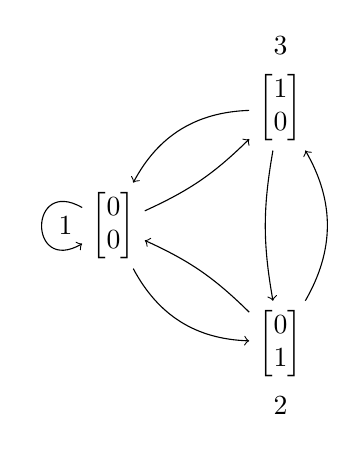
\begin{tikzpicture}[scale=1.5]
            \node[label=left:$1$] (1) at (0,0) {$\begin{bmatrix}0 \\ 0\end{bmatrix}$};
            \node[label=below:$2$] (3) at ({sqrt(2)},-1) {$\begin{bmatrix}0 \\ 1\end{bmatrix}$};
            \node[label=$3$] (2) at ({sqrt(2)},1) {$\begin{bmatrix}1 \\ 0\end{bmatrix}$};

            \draw[->] (1) to[out=150, in=210, distance=1.5em] (1);
            \draw[->] (1) to[bend right=10] (2);
            \draw[->] (1) to[bend right] (3);
            \draw[->] (3) to[bend right] (2);

            \draw[->] (2) to[bend right] (1);
            \draw[->] (2) to[bend right=10] (3);
            \draw[->] (3) to[bend right=10] (1);
        \end{tikzpicture}
    \end{center}

    The adjacency matrix for the graph is
    \begin{equation*}
        A = \begin{bmatrix}
            1 & 1 & 1 \\
            1 & 0 & 1 \\
            1 & 1 & 0
        \end{bmatrix}
    \end{equation*}

    The generating function for the number of combinations is then the sum of all entries in 
\begin{equation*}
        B=(I-xA)^{-1}
\end{equation*}
however we need to account for the fact that the walks of length $0$ are the combinations counted in $a(2, 1)$.

\newpage

\section*{Problem 2.7}
\paragraph{Description:}
Each of $n$ (distinguishable) telephone poles is painted red, blue, or any of an additional $k$ colours. Determine the number of ways this can be done so that an odd number are painted red and an even number blue.

\paragraph{Solution:}
If we represent whether the red and blue poles are odd or even with a $1$ or $0$, we can represent their state with a $2$-bit binary string where the first bit represents red and the second one blue (read from left to right). Thus we get the DFA

\begin{center}
    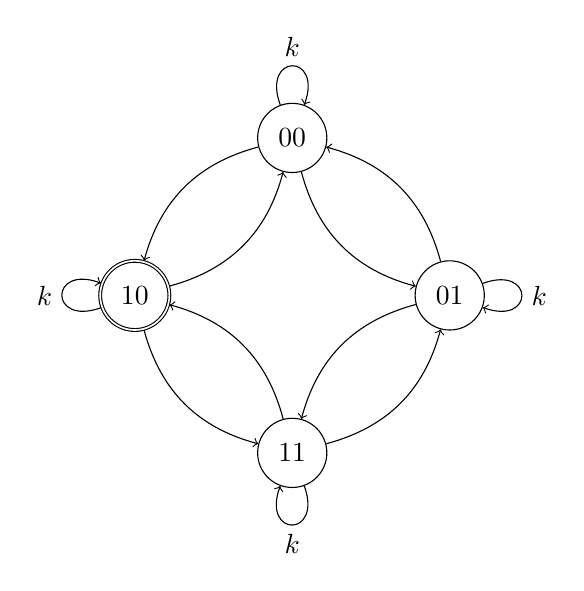
\begin{tikzpicture}[scale=2]
        \node[state, accepting] (0) at (0, 0) {$10$};
        \node[state] (1) at (1, 1) {$00$};
        \node[state] (2) at (1, -1) {$11$};
        \node[state] (3) at (2, 0) {$01$};

        \draw[->] (0) to[out=200, in=160, distance=1em] node[midway, left] {$k$} (0);
        \draw[->] (1) to[out=110, in=70, distance=1em] node[midway, above] {$k$} (1);
        \draw[->] (2) to[out=-70, in=-110, distance=1em] node[midway, below] {$k$} (2);
        \draw[->] (3) to[out=20, in=-20, distance=1em] node[midway, right] {$k$} (3);

        \draw[->] (0) to[bend right] (1);
        \draw[->] (0) to[bend right] (2);
        \draw[->] (1) to[bend right] (0);
        \draw[->] (1) to[bend right] (3);
        \draw[->] (2) to[bend right] (0);
        \draw[->] (2) to[bend right] (3);
        \draw[->] (3) to[bend right] (1);
        \draw[->] (3) to[bend right] (2);
    \end{tikzpicture}
\end{center}

The adjacency matrix representing this digraph is
\begin{equation*}
    A = \begin{bmatrix}
        k & 1 & 1 & 0 \\
        1 & k & 0 & 1 \\
        1 & 0 & k & 1 \\
        0 & 1 & 1 & k
    \end{bmatrix}
\end{equation*}

The generating function for walks of length $n$ that start and end at the accepted state would be the sum of the entries in row $1$ of $B=(I-xA)$, that is
\begin{equation*}
    F(x) = \frac{1-2kx+(k^2-2)x^2}{1-3kx + (3k^2-4)x^2-(k^3-4k)x^3}
\end{equation*}

\end{document}
